\documentclass[11pt]{article}
\usepackage{geometry}                
\geometry{letterpaper,tmargin=1in,bmargin=1in,lmargin=1in,rmargin=1in} 
\usepackage[parfill]{parskip}    % Activate to begin paragraphs with an empty line rather than an indent
\usepackage{graphicx}
\usepackage{amsmath, amsfonts, amsthm, amssymb} 
\usepackage[shortlabels]{enumitem}
\usepackage{xcolor}
\usepackage{mathtools}

\parskip = 0.1in

\pagestyle{myheadings}
\markright{Homework of IOE 611 Nonlinear Programming\hfill Yulun Zhuang \hfill}

 % some traditional definitions that can be blamed on craig barratt
 \newcommand{\BEAS}{\begin{eqnarray*}}
\newcommand{\EEAS}{\end{eqnarray*}}
\newcommand{\BEA}{\begin{eqnarray}}
\newcommand{\EEA}{\end{eqnarray}}
\newcommand{\BEQ}{\begin{equation}}
\newcommand{\EEQ}{\end{equation}}
\newcommand{\BIT}{\begin{itemize}}
\newcommand{\EIT}{\end{itemize}}

% text abbrevs
\newcommand{\eg}{e.g.}
\newcommand{\ie}{i.e.}

% std math stuff
\newcommand{\ones}{\mathbf 1}
\newcommand{\real}{{{\mathbb{R}}}}
\newcommand{\integer}{{{\mathbb{Z}}}}
\newcommand{\complex}{{{\mathbb{C}}}}
\newcommand{\symm}{{{\mathbb{S}}}}  % symmetric matrices
%
% lin alg stuff
\newcommand{\Span}{\mbox{\textrm{span}}}
\newcommand{\range}{{\mathcal R}}
\newcommand{\nullspace}{{\mathcal N}}
\newcommand{\Rank}{\mathop{\textbf{rank}}}
\newcommand{\Tr}{\mathop{\textbf{tr}}}
\newcommand{\cond}{\mathop{\textbf{cond}}}
\newcommand{\diag}{\mathop{\textbf{diag}}}
\newcommand{\lambdamax}{\lambda_{\rm max}}
\newcommand{\lambdamin}{\lambda_{\rm min}}

% probability stuff
\newcommand{\Prob}{\mathop{\textbf{prob}}}
\newcommand{\Expect}{\mathop{\textbf{E{}}}}
\newcommand{\var}{\mathop{\textbf{var}}} % variance
% not sure why we have \Expect and \Prob but \var ???

% convexity & optimization stuff
\newcommand{\Co}{\mathop {\textbf{conv}}} % convex hull
\newcommand{\argmin}{\mathop{\rm argmin}}
\newcommand{\argmax}{\mathop{\rm argmax}}
\newcommand{\epi}{\mathop{\textbf{epi}}}
%\newcommand{\hypo}{\mathop{\textbf{hypo}}}}

% sup and inf that look OK in saddle-point form!
%\newcommand{\ourinf}{\mathop{\raisebox{0ex}[0ex][.4ex]{\,inf\,}}}
%\newcommand{\oursup}{\mathop{\raisebox{0ex}[0ex][.4ex]{\,sup\,}}}
\newcommand{\ourinf}{\mathop{\,\mathrm{inf}\, {\rule[-.5ex]{0ex}{0ex}}}}
\newcommand{\oursup}{\mathop{\,\mathrm{sup}\, {\rule[-.5ex]{0ex}{0ex}}}}
%makes latex believe that inf and sup both extend .4ex below
%the baseline

\newcommand{\dist}{\mathop{\textbf{dist}}}
\newcommand{\vol}{\mathop{\textbf{vol}}} % volume
\newcommand{\Card}{\mathop{\textbf{card}}} % cardinality
\newcommand{\sign}{\mathop{\textbf{sign}}}

\newcommand{\dom}{\mathop{\textbf{dom}}} % domain
\newcommand{\aff}{\mathop{\textbf{aff}}} % affine hull
\newcommand{\cl}{\mathop{\textbf{cl}}} % closure
\newcommand{\intr}{\mathop{\textbf{int}}} % interior
\newcommand{\relint}{\mathop{\textbf{rel int}}} % relative interior
\newcommand{\bd}{\mathop{\textbf{bd}}} % boundary

%why do we have the following but not \nust?
\newcommand{\xst}{x^\star}
\newcommand{\lambdast}{\lambda^\star}

% defs for cones & generalized inequalities
% these seem kind of awkward; should fix some day
% rewrite them to use args?
\newcommand{\geqK}{\mathrel{\succeq_K}}
\newcommand{\gK}{\mathrel{\succ_K}}
\newcommand{\leqK}{\mathrel{\preceq_K}}
\newcommand{\lK}{\mathrel{\prec_K}}
\newcommand{\geqKst}{\mathrel{\succeq_{K^*}}}
\newcommand{\gKst}{\mathrel{\succ_{K^*}}}
\newcommand{\leqKst}{\mathrel{\preceq_{K^*}}}
\newcommand{\lKst}{\mathrel{\prec_{K^*}}}
\newcommand{\geqL}{\mathrel{\succeq_L}}
\newcommand{\gL}{\mathrel{\succ_L}}
\newcommand{\leqL}{\mathrel{\preceq_L}}
\newcommand{\lL}{\mathrel{\prec_L}}
\newcommand{\geqLst}{\mathrel{\succeq_{L^*}}}
\newcommand{\gLst}{\mathrel{\succ_{L^*}}}
\newcommand{\leqLst}{\mathrel{\preceq_{L^*}}}
\newcommand{\lLst}{\mathrel{\prec_{L^*}}}

%\newcounter{lecture}
%\newcommand{\lecturefl}[1]{   % use with foiltex landscape
%% \addtocounter{lecture}{1}
% \refstepcounter{lecture}
% \setcounter{equation}{0}
% \setcounter{page}{1}
% \renewcommand{\theequation}{\arabic{equation}}
% \renewcommand{\thepage}{\arabic{lecture}--\arabic{page}}
% \raggedright
% \parindent 0pt
% \rightfooter{\thepage}
% \leftheader{}
% \rightheader{}
% \LogoOff
% \input header 
% \begin{center}
%% {\Large \bfseries Lecture \arabic{lecture} \\*[\bigskipamount] {#1}}
%{\Large \bfseries \arabic{lecture}.  {#1}}
% \end{center}
% \MyLogo{#1}
%}

%\newcommand{\lectureflstar}[1]{   % use with foiltex landscape
% \setcounter{equation}{0}
% \setcounter{page}{1}
% \renewcommand{\theequation}{\arabic{equation}}
% \renewcommand{\thepage}{\arabic{page}}
% \raggedright
% \parindent 0pt
% \rightfooter{\thepage}
% \leftheader{}
% \rightheader{}
% \LogoOff
% \input header 
% \begin{center}
% {\Large \bfseries #1}
% \end{center}
% \MyLogo{#1}
%}
%\newcounter{oursection}
%\newcommand{\frametitle}[1]{  % for use with foiltex landscape
% \addtocounter{oursection}{1}
%% \setcounter{equation}{0}
% \foilhead[-1.0cm]{#1}
% \LogoOn
%}

\newenvironment{algdesc}%
   {\begin{list}{}{%
   \setlength{\rightmargin}{0\linewidth}%
   \setlength{\leftmargin}{.05\linewidth}}%
   \sffamily\small
   \item[]{\setlength{\parskip}{0ex}\hrulefill\par%
   \nopagebreak{}}}%
   {{\setlength{\parskip}{-1ex}\nopagebreak\par\hrulefill} \end{list}}

\newenvironment{colm}{\left[\begin{array}{c}}{\end{array}\right]}
\newenvironment{colv}{\left(\begin{array}{c}}{\end{array}\right)}


\newcommand{\oh}{\frac12}
\newcommand{\st}{\text{subject to}}
\newcommand{\gfb}{\nabla f(\bar x)}
\newcommand{\hfb}{H(\bar x)}

\newtheorem{theorem}{Theorem}[section]
\newtheorem{remark}[theorem]{Remark}%[section]
\newtheorem{definition}[theorem]{Definition}%[section]
\newtheorem{proposition}[theorem]{Proposition}%[section]
\newtheorem{lemma}[theorem]{Lemma}%[section]
\newtheorem{corollary}[theorem]{Corollary}%[section]
\newtheorem{assumption}{Assumption}
\newtheorem{claim}{Claim}
\newtheorem{exam}{Example}
\newenvironment{solution}
  {\renewcommand\qedsymbol{$\square$}\begin{proof}[\textbf{Solution}]}
  {\end{proof}}
\renewcommand{\proofname}{\textbf{Proof}}

\newcommand{\red}[1]{\textcolor{red}{#1}}
\newcommand{\blue}[1]{\textcolor{blue}{#1}}
\newcommand{\green}[1]{\textcolor{green}{#1}}
\newcommand{\grad}{\nabla}
\newcommand{\hess}{\nabla^2}
\newcommand{\tr}{\text{tr}}

\newcommand{\dd}{\mathrm{d}}
\newcommand{\RR}{\mathbb{R}}
\newcommand{\NN}{\mathbb{N}}
\newcommand{\ZZ}{\mathbb{Z}}
\newcommand{\bS}{\mathbb{S}}

\newcommand{\pd}[2][]{ \frac{\partial #1}{\partial #2}} % Partial derivatives
\renewcommand{\d}{{\rm d}}
\newcommand{\ddt}{\frac{\d}{\d t}}
\newcommand{\half}{\frac{1}{2}}
\newcommand{\inv}{^{-1}}
\newcommand{\T}{^\top}

\begin{document}
\title{IOE 611: Homework 4}
\author{Yulun Zhuang}
\maketitle
%**********************************
\section*{Problem 1}
Each of the following \texttt{cvx} code fragments describes a convex constraint on the scalar variables $x$, $y$, and $z$, but violates the \texttt{cvx} rule set, and so is invalid. Briefly explain why each fragment is invalid. Then, rewrite each one in an equivalent form that conforms to the \texttt{cvx} rule set.

(a) \texttt{norm([x + 2*y, x - y]) == 0} is invalid because the equality constraints have to be affine for the problem to be convex. Since $\|v\|=0$ if and only if $v = 0$ element-wise, the constraint can be reformulated as
\begin{align*}
    &\texttt{x + 2*y == 0;} \\
    &\texttt{x - y == 0;}
\end{align*}

(b) \texttt{square(square(x + y)) <= x - y} is invalid because the convexity of a square function of a convex function can not be determined. The square of square is equivalent to the fourth power, 
\begin{align*}
    \texttt{power(x + y, 4) <= x - y;}
\end{align*}

(c) \texttt{1/x + 1/y <= 1; x >= 0; y >= 0} is invalid because $1/x$ is not convex without restricting the domain to $\real_{++}$. It can be reformulated as
\begin{align*}
    &\texttt{inv\_pos(x) + inv\_pos(y) <= 1;}
\end{align*}

(d) \texttt{norm([max(x, 1), max(y, 2)]) <= 3*x + y} is invalid because the convexity of the norm of a convex function is undetermined. Introduce and minimize over additional variables $[u, v]$ which is convex and non-decreasing over its domain
\begin{align*}
    &\texttt{norm([u, v]) <= 3*x + y;} \\
    &\texttt{u >= max(x, 1)}\\
    &\texttt{v >= max(y, 2)}
\end{align*}

(e) \texttt{x*y >= 1; x >= 0; y >= 0} if invalid because \texttt{x*y} is nonlinear. However, given the variables are both positive from the combination of constraints, it can be reformulated as
\begin{align*}
    &\texttt{y >= inv\_pos(x)}
\end{align*}

(f) \verb|(x + y)^2 / sqrt(y) <= x - y + 5| is invalid because LHS is convex function over concave function, which has undetermined convexity. It can be reformulated as a quadratic term over a nonincreasing linear term as
\begin{align*}
    &\texttt{quad\_over\_lin(x + y, sqrt(y)) <= (x - y + 5)} 
\end{align*}

(g) \verb|x^3 + y^3 <= 1; x >= 0; y >= 0| is invalid because $x^3$ is not convex. Instead, use $\texttt{pow\_pos(x, p)}$
\begin{align*}
    &\texttt{pow\_pos(x, 3) + pow\_pos(y, 3) <= 1;}
\end{align*}

(h) \verb|x + z <= 1 + sqrt(x*y - z^2); x >= 0; y >= 0| is invalid because \texttt{x*y} is nonlinear. Observe that 
\begin{align*}
    \sqrt{xy - z^2} = \left( \det 
    \begin{bmatrix}
        x & z \\
        z & y
    \end{bmatrix} \right) ^{1/2}
\end{align*}
The constraint is equivalent to 
\begin{align*}
    &\texttt{x + z <= 1 + det\_rootn([x, z; z, y]);} \\
    &\texttt{x >= 0; y >= 0;}
\end{align*}
where for $X\in \real^{n \times n}$, $\texttt{det\_rootn(X)} = \det(X)^{1/n}$.



\clearpage
\section*{Problem 2}
Consider a two-dimensional bounded object $R \subset \real^2$ that has density $\rho (z)$ at point $z = (x, y) \in \real^2$. Then the mass $m \in \real$, center of gravity $c \in \real^2$, and inertia matrix $M \in\real^{2\times 2}$ of this object are given by, respectively,
\[
m = \int_{R} \rho (z) dxdy,\ c=\frac{1}{m} \int_R \rho (z) z dxdy,\ M = \int_R \rho (z) (z - c)(z-c)\T dxdy
\]

(a) Suppose $R$ is discretized into $n$ pixels, each of area $a$, with pixel $i$ having constant density $\rho_i$ throughout and location (say, of its center) $z_i \in\real^2$. Replace expressions for $m$, $c$, and $M$ with sums and averages using this discretization.

(b) Formulate the following as a convex optimization problem: choose the density vector $\rho$ in order to maximize $\lambda_{\min}(M)$, subject to $0 \leq \rho(z) \leq \rho_{\max}$ for all $z \in\real$, and a fixed total mass $m = m_{\text{given}}$.

(c) Apply your method to the instance with data in \texttt{hwk4p2data.m}.


\begin{solution}
  (a) 
  \begin{align*}
    m &= a\sum_{i=1}^{n} \rho_i\\
    c &= \frac{a}{m} \sum_{i=1}^{n} \rho_i z_i\\
    M &= a \sum_{i=1}^{n} \rho_i (z_i - c) (z_i - c)\T
  \end{align*}

  (b) Given that $\lambda_{\min}(M) \geq t \Leftrightarrow M \succeq tI$, the problem can be formulated as
  \begin{align*}
    \max_{\rho, t} \quad & t\\
    \text{s.t.}\quad 
    & a \sum_{i=1}^{n} \rho_i (z_i - c) (z_i - c)\T \succeq tI\\
    & c = \frac{a}{m_{\text{given}}} \sum_{i=1}^{n} \rho_i z_i\\
    & a\sum_{i=1}^{n} \rho_i = m_{\text{given}}\\
    & 0 \leq \rho_i \leq \rho_{\max},\ i=1, \dots, n
  \end{align*}

  Note that $M$ can be further simplified as
  \begin{align*}
    M 
    &=  a \sum_{i=1}^{n} \rho_i (z_i - c) (z_i - c)\T\\
    &= a \sum_{i=1}^{n} \rho_i (z_i z_i\T -c z_i\T -z_i c\T + cc\T)\\
    &= a \sum_{i=1}^{n} \rho_i z_i z_i\T - a c \sum_{i=1}^{n} (\rho_i z_i)\T - a (\sum_{i=1}^{n} \rho_i z_i)c\T + cc\T a \sum_{i=1}^{n} \rho_i\\
    &= a \sum_{i=1}^{n} \rho_i z_i z_i\T - m_{\text{given}} cc\T
  \end{align*}

  Now we work on the only nonlinear constraint. By using the Schur complement theorem, this constraint can be reformulated as
  \begin{align*}
    &(a \sum_{i=1}^{n} \rho_i z_i z_i\T - tI) - m_{\text{given}} cc\T \succeq 0\\
    \Leftrightarrow\  &\begin{bmatrix}
      a \sum_{i=1}^{n} \rho_i z_i z_i\T - tI & c\T\\
      c & 1/m_{\text{given}}
    \end{bmatrix}
    \succeq 0
  \end{align*}
  which is a Linear Matrix Inequality (LMI) in $\rho, t$.

  (c) The optimal inertia matrix is
  \[
    M^* = \begin{bmatrix}
      0.6484  & -0.0000\\
      -0.0000 &  0.6484
    \end{bmatrix}
  \]
  \begin{figure}[htb]
    \centering
    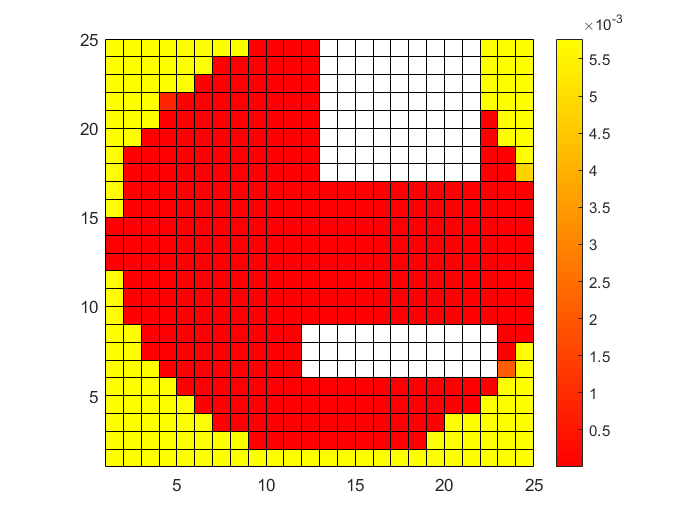
\includegraphics[width=0.5\columnwidth]{hw4p2.png}
    \caption{Visualization of the optimal density distribution.}
    \label{fig:p2}
  \end{figure}

\end{solution}


\clearpage
\section*{Problem 3}
Implement the SDP relaxation of the Max-Cut problem.

(a) Use your code to solve an instance of the problem with a weight matrix provided in \texttt{hw4p3data1.m}. Plot the distribution of the eigenvalues of Y. Is your SDP relaxation exact? If yes, recover the optimal solution for the Max-Cut problem from Y. If no, explain why.

(b) Use your code to solve an instance of the problem with a weight matrix provided in \texttt{hw4p3data2.m}. Plot the distribution of the eigenvalues of Y. Is your SDP relaxation exact? If yes, recover the optimal solution for the Max-Cut problem from Y. If no, explain why.

\begin{solution}
  (a) The SDP relaxation is not exact since the number of nonzero eigenvalues of Y is more than 1, i.e. the rank of Y is greater than 1.
  \vspace{-1em}
  \begin{figure}[htb]
    \centering
    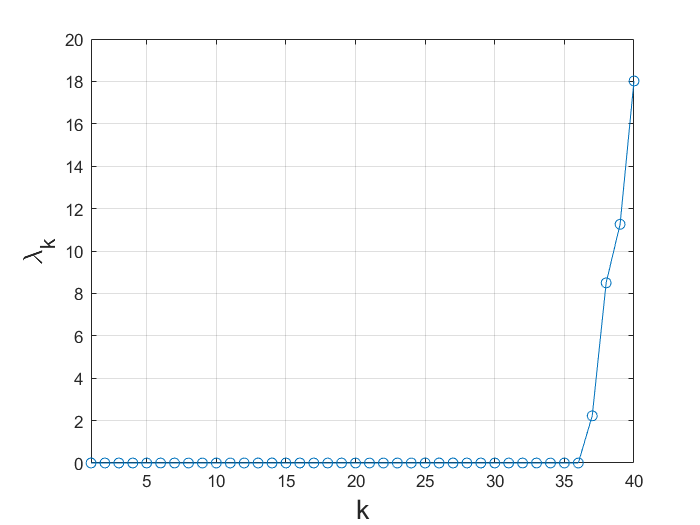
\includegraphics[width=0.45\columnwidth]{hw4p3a.png}
    \caption{Eigenvalues of Y for \texttt{data1}}
    \label{fig:p3a}
  \end{figure}

  (b) The SDP relaxation is exact since the number of nonzero eigenvalues of Y is equal to 1 i.e. the rank of Y is equal to 1.
  \vspace{-1em}
  \begin{figure}[htb]
    \centering
    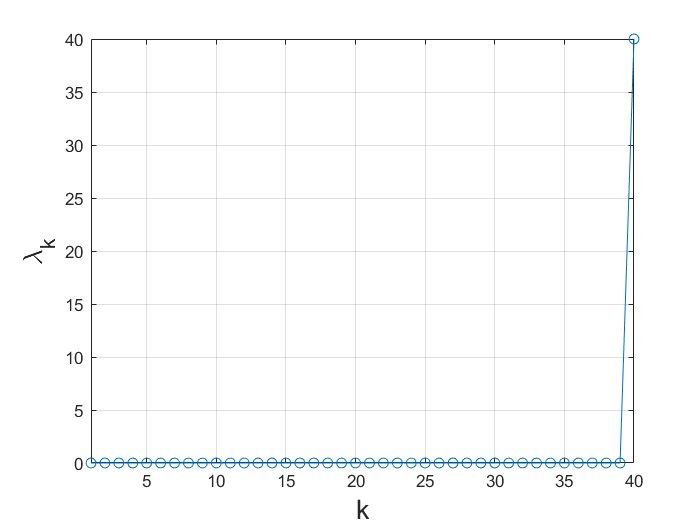
\includegraphics[width=0.45\columnwidth]{hw4p3b.png}
    \caption{Eigenvalues of Y for \texttt{data2}}
    \label{fig:p3b}
  \end{figure}

  The recovered solution is 
  \[
  x = \sqrt{\lambda_{40}} v_{40} = [-\ones_{1\times 20}, \ones_{1\times 20}]\T
  \]
\end{solution}


\clearpage
\section*{Problem 4}
\textit{Weak duality for unbounded and infeasible problems}. 
The weak duality inequality, $d^* \leq p^*$,
clearly holds when $d^* = -\infty$ or $p^* = \infty$. Show that it holds in the other two cases as well: If $p^* = -\infty$, then we must have $d^* = -\infty$, and also, if $d^* = \infty$, then we must have $p^* = \infty$.

\begin{proof}
  (a) 
  If $p^* = -\infty$, then the primal problem is unbounded below. In other words, there exists feasible $x$ that makes $f_0(x) \to -\infty$. Then, for the dual function with $\lambda_i \geq 0$ for $i = 1, \ldots, m$, 
  \begin{align*}
      g(\lambda, \nu) 
      &= \inf_x f_0(x) + \sum_{i=1}^m \lambda_i f_i(x) + \sum_{i=1}^p \nu_i h_i(x) \\
      &= -\infty + \inf_x\sum_{i=1}^m \lambda_i f_i(x) + \sum_{i=1}^p \nu_i h_i(x) \\
      &= -\infty
  \end{align*}
  Since the above holds for all feasible $(\lambda, \nu)$, 
  \begin{align*}
      d^* = \max g(\lambda, \nu) = - \infty
  \end{align*}
  
  (b)
  To prove by contradiction, assume $p^* \neq \infty$, which implies that $p^*$ is feasible. Therefore there exists $\bar{x}$ such that
  \begin{align*}
      L(\lambda, \nu, \bar{x}) = f_0(\bar{x}) + \sum_{i=1}^m \lambda_i f_i(\bar{x}) + \sum_{i=1}^p \nu_i h_i(\bar{x})
  \end{align*}
    is obtained with $f_i(\bar{x}) \leq 0$ for $i = 1, \ldots, m$ and $h_i(\bar{x}) = 0$ for $i = 1, \ldots, p$. $L(\lambda, \nu, \bar{x})$ can be an upper bound for $g$, which is the infimum of $L$, 
  \begin{align*}
      g(\lambda, \nu) 
      = \inf_x f_0(x) + \sum_{i=1}^m \lambda_i f_i(x) + \sum_{i=1}^p \nu_i h_i(x) 
      \leq L(\lambda, \nu, \bar{x})
  \end{align*}
  Therefore, if $p^* \neq \infty$, $d^* = \max g(\lambda, \nu) = \infty$ is not true since $g(\lambda, \nu)$ is bounded above. Then, by contradiction, if $g=\infty$, then $p^* = \infty$.
\end{proof}

\clearpage
\section*{Problem 5}
\textit{Suboptimality of a simple covering ellipsoid}. 
Recall the problem of determining the minimum
volume ellipsoid, centered at the origin, that contains the points $a_1, \dots, a_m\in\real^n$
\begin{align*}
  \text{minimize}\quad& f_0(X) = \log\det(X^{-1})\\
  \text{subject to}\quad & a_i\T X a_i \leq 1, \ i=1,\dots, m,
\end{align*}
with $\dom f_0 = \symm^n_{++}$.
We assume that the vectors $a_1, \dots, m \text{ span } \real^n$ (which implies that the problem is bounded below).

(a) Show that the matrix
\[
X_{sim} = \left(\sum_{k=1}^{m}a_ka_k\T\right)^{-1},
\]
is feasible.

(b) Now we establish a bound on how suboptimal the feasible point $X_{sim}$ is, via the dual
problem,
\begin{align*}
  \text{minimize}\quad& \log\det(\sum_{i=1}^{m} \lambda_i a_i a_i\T) - \ones\T \lambda + n\\
  \text{subject to}\quad & \lambda \succeq 0,
\end{align*}
with the implicit constraint $\sum_{i=1}^{m} \lambda_i a_i a_i\T \succ 0$.
To derive a bound, we restrict our attention to dual variables of the form $\lambda = t\ones$, where $t > 0$. Find (analytically) the optimal value of $t$, and evaluate the dual objective at this $\lambda$. Use this to prove that the volume of the ellipsoid $\{u\mid u\T X_{sim}u\leq 1\}$ is no more than a factor $(m/n)^{n/2}$ more than the volume of the minimum volume ellipsoid.

\begin{proof}
  (a)
  \begin{align*}
    \begin{bmatrix}
    \sum_{k=1}^m a_k a_k^\top & a_i \\
    a_i & 1
    \end{bmatrix}
    =
    \sum_{k}
    \begin{bmatrix}
    a_k \\
    0
    \end{bmatrix}
    \begin{bmatrix}
    a_k \\
    0
    \end{bmatrix}^\top +
    \begin{bmatrix}
        a_i \\ 1
    \end{bmatrix} 
    \begin{bmatrix}
        a_i \\ 1
    \end{bmatrix}^\top
  \end{align*}
  where $k = 1, \ldots, m$ and $k \neq i$. Each of the term is in the form of $V^\top V$ and therefore is PSD. Hence, $Z \succeq 0$ because it is a sum of PSDs. 
  
  Let $A = \sum_{k=1}^m a_k a_k^\top, B = a_i, C = 1$, then based on Schur complements, since $Z \succeq 0$, 
  \begin{align*}
      C - B^\top A^{-1} B &\geq 0 \\
      1 - a_i^\top \left( \sum_{k=1}^m a_k a_k^\top \right)^{-1} a_i &\geq 0 \\
      a_i^\top X_{\text{sim}} a_i &\leq 1
  \end{align*}
  for $i = 1, \ldots, m$. Therefore, $X_{\text{sim}}$ is feasible. 

  (b)
  Firstly, for $X = X_\text{sim}$, the primal objective value is 
  \begin{align*}
      f_0(X_\text{sim}) = \log \det(X_\text{sim}^{-1}) = \log \det \left( \sum_{k=1}^m a_k a_k^\top \right)
  \end{align*}
  Then, to derive the bound via dual with $\lambda = t\mathbf{1}$, 
  \begin{align*}
      L(\lambda = t\textbf{1}) =& \log \det \left( \sum_{i=1}^m t a_i a_i^\top \right) - \mathbf{1}^\top t \textbf{1} + n \\
      =& \log \left( t^n \det \left( \sum_{i=1}^m a_i a_i^\top \right) \right) - mt + n \\
      =& \log \det \left( \sum_{i=1}^m a_i a_i^\top \right) + n\log(t) - mt + n
  \end{align*}
  To derive the optimal $t^*$ for the dual problem, find the derivative and set it to zero, 
  \begin{align*}
      \frac{dL}{dt} &= \frac{n}{t} - m = 0 \\
      t^* &= \frac{n}{m}
  \end{align*}
  Substituting to $L(\lambda = t\textbf{1})$, the dual objective value is  
  \begin{align*}
      g(t\mathbf{1}) = \log \det \left( \sum_{i=1}^m a_i a_i^\top \right) + n\log\left(\frac{n}{m}\right)
  \end{align*}
  The duality gap, $f_0(X_\text{sim}) - g(t\mathbf{1})$, is 
  \begin{align*}
    \log \det \left( \sum_{i=1}^m a_i a_i^\top \right) - \log \det \left( \sum_{i=1}^m a_i a_i^\top \right) - n\log\left(\frac{n}{m}\right) = n\log\left(\frac{m}{n}\right)
  \end{align*}
  which means $X_\text{sim}$ is at most $n\log\left(\frac{m}{n}\right)$ larger than the optimal primal objective. The volume of the ellipsoid $\mathcal{E}_x = \{z \mid z^\top X z \leq 1\}$ is proportional to $(\det X^{-1})^{1/2}$, which can be transformed from the primal by multiplying by $1/2$ and taking the exponential, 
  \begin{align*}
      \exp(2 f_0) = \exp\left(\frac{1}{2}\log \det(X^{-1})\right) = (\det X^{-1})^{1/2}
  \end{align*}
  Applying the same transformation to the duality gap, 
  \begin{align*}
      \exp\left( \frac{n}{2} \log\left(\frac{m}{n}\right) \right) = \left(\frac{m}{n}\right)^{n/2}
  \end{align*}
  Therefore, the volume of the ellipsoid with $X_\text{sim}$ is no more than a factor of $\left(\frac{m}{n}\right)^{n/2}$ more than that of the minimum volume ellipsoid. 

\end{proof}

\end{document}
